
\section{Trénovacie dáta}
\label{sec:trenovaciedata}

\subsection{Zber dát}
Pre trénovanie modelov boli použité obrázky zo zdrojov spomenutých v~kapitole \ref{sec:databaza}.
Tabuľka nižšie uvádza podrobné počty obrázkov z~daných zdrojov, ktoré boli použité pre určenie typu zbrane v~2 kategóriách.

\begin{table}[H]
  \centering
  \label{my-label}
  \begin{tabular}{|l|c|c|}
    \hline
    Zdroj               & \multicolumn{1}{l|}{Počet krátkych zbraní} & \multicolumn{1}{l|}{Počet dlhých zbraní} \\ \hline
    IMFDB               & 647                                        & 670                                      \\ \hline
    ImageNet            & 730                                        & 94                                       \\ \hline
    Google vyhľadávanie & 0                                          & 86                                       \\ \hline \hline
    SPOLU               & 1377                                       & 850                                      \\ \hline
  \end{tabular}
  \caption{Podrobné počty trénovacích dát.}
\end{table}

Vo všeobecnosti je jednoduchšie nájsť obrázky, ktoré obsahujú krátke zbrane (pištole) ako dlhé zbrane.
Databáza ImageNet obsahovala vyše 3000 odkazov na obrázky, avšak veľká časť z~nich bola chybná alebo daný súbor už neexistoval.

Ako bolo spomínané v~\ref{subsec:generovanie3d}, obrázky ktoré boli použité na trénovanie modelov pre určenie náklonu zbrane bolo potrebné
    vygenerovať pomocou 3D modelov.
Pre toto generovanie bolo použitých desať pozadí scény a päť 3D modelov z~toho tri modely boli dlhé zbrane a dve modely krátkych zbraní.

\begin{figure}[H]
    \centering
    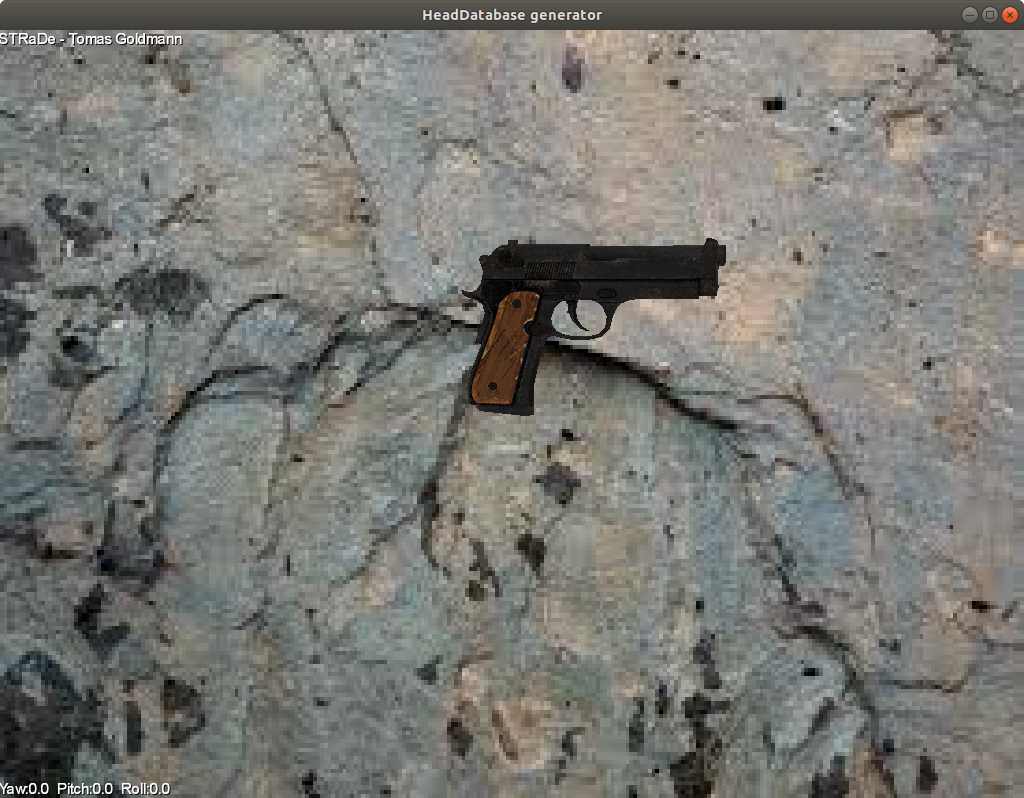
\includegraphics[width=0.7\textwidth]{generator3d}
    \caption{Program pre generovanie obrázkov z~3D modelov.}
    \label{pic:generator3d}
\end{figure}

Niektoré použité modely mali nastavený zlý bod otáčania a taktiež boli veľmi malé.
Preto, ako je vidieť na obrázku \ref{pic:generator3d}, museli byť výsledne obrázky ešte orezané aby sa v~nich nachádzala iba zbraň bez nepotrebného okolia.

\begin{figure}[H]
    \centering
    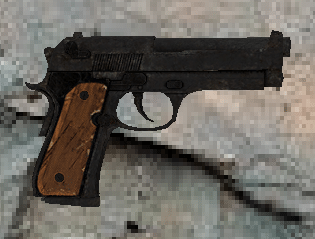
\includegraphics[width=0.5\textwidth]{croped_weapon}
    \caption{Výsledný vygenerovaný obrázok po orezaní okolia.}
    \label{pic:generator3d}
\end{figure}

Tabuľka nižšie uvádza presné počty vygenerovaných obrázkov.

\begin{table}[H]
    \centering
    \label{my-label}
    \begin{tabular}{|l|c|}
        \hline
        Typ osi otáčania & \multicolumn{1}{l|}{Počet obrázkov} \\ \hline
        pitch            & 1480                                \\ \hline
        roll             & 4450                                \\ \hline
        yaw              & 4600                                \\ \hline
        \end{tabular}
    \caption{Podrobné počty trénovacích dát.}
\end{table}

Pre os otáčania pitch boli vybrané obrázky z~datasetu určeného pre klasifikáciu typu zbrane.
Pre zvyšné 2 osi boli obrázky generované, počty sa líša kvôli niektorým chybným obrázkom, ktoré museli byť vymazané.

\subsection{Načítavanie dát}
\label{subsec:nacitaniedat}
Pre načítavanie dát je implementovaná trieda \textit{DataLoader} v~scripte \textit{loader.py}.
Trieda obsahuje niekoľko funkcií pre načítanie týchto dát, tieto funkcie vrátia pole načítaných obrázkov, pole indexov označení (angl. \textit{labels}) obrázkov a
    slovník, ktorý obsahuje index a názov označenia, napr. \{0: ``kratka zbran'', 1: ``dlha zbran''\}.

Prvá z~funkcií načítava dáta z~priečinka, kde označenie obrázkov, či je to krátka alebo dlhá zbraň, je zabezpečené podľa názvov podpriečinkov.
Pre obrázky o~náklone zbrane sa označenie osi berie tiež z~názvu podpriečinka, avšak presné označenie o~koľko stupňov je model v~obrázku otočený
    sa získa z~názvu obrázka, ktorý musí spĺnať presný formát: \textit{p0.0\_y0.0\_r0.0-typzbrane.jpg}.
Kde \textit{p0.0} označuje hodnotu náklonu v~osi pitch, \textit{y0.0} hodnotu náklonu v~osi yaw, \textit{r0.0} v~osi roll a \textit{typzbrane} môže byť
    akýkoľvek reťazec.
Formát vstupných obrázkov môže byť \textit{.jpg} alebo \textit{.jpeg}.

Správnu hierarchiu priečinkov je vidieť na obrázku \ref{pic:folderhierarchy}.

\begin{figure}[H]
    \centering
    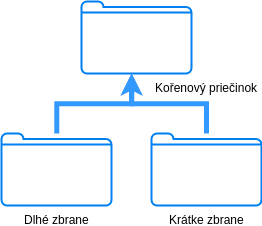
\includegraphics[width=0.32\textwidth]{class_hierarchy}
    \qquad
    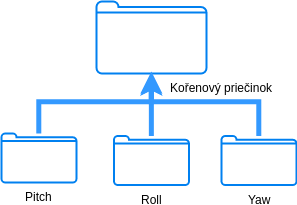
\includegraphics[width=0.4\textwidth]{angle_hierarchy}
    \caption{Hierarchia priečinkov pre správne označenie vstupných obrázkov.}
    \label{pic:folderhierarchy}
\end{figure}

Druhá z~funkcií umožňuje načítať zoznam obrázkov z~textového súboru, kde sa na každom riadku nachádza práve jedna cesta k~požadovanému obrázku.
Spôsob označovania obrázkov je rovnaký ako v~prvom prípade, preto je taktiež potrebné dodržať správnu hierachiu priečinkov.

\subsection{Predspracovanie dát}
\label{subsec:predspracovaniedat}
Pre predspracovanie obrazu sú implementované 2 triedy \textit{Preprocessor} a \textit{Preprocessing} v~scripte \textit{preprocessing.py}.
Trieda \textit{Preprocessor} obsahuje list, do ktorého je možné pridávať funkcie, ktoré sú implementované v~triede \textit{Preprocessing}.
Po zavolaní funkcie \textit{apply(input\_data)} z~triedy \textit{Preprocessor}, sa tieto
    funkcie v~poradí, v~akom boli pridané do listu zavolajú a prebehne predspracovanie vstupných dát.
Každá z~možností predspracovanie obrazu, ktorá bola uvedená v~\ref{sec:preprocessing}, je implementovaná v~triede \textit{Preprocessing}, v~samostatnej funkcii,
    pomocou knižnice scikit-image.

Pre augmentáciu dát určených na klasfikáciu typu zbrane je použitá trieda \textit{ImageDataGenerator} z~knižnice Keras.
Parametre tohto generátora sú nastavené na: horizonálne a vertikálne preklopenia obrázka, posun obrázka až o~15\% jeho dĺžky alebo šírky,
    rotácia o~náhodný uhol v~rozsahu 0 až 180 stupňov a doplnenie čiernych pixelov pomocou nastavenia ``nearest''.

Pre augmentáciu dát, pre určenie náklonu zbrane je implementovaná samostatná trieda \textit{AngleGenerator}, ktorá zabezpečuje správne dogenerovanie
    vstupných dát pomocou horizontálneho alebo vertikálneho preklopenia obrázka a správneho výpočtu uhla natočenia (viď. \ref{subsec:augmentacia}).
